\documentclass[../AnalysisNoteJBuxton.tex]{subfiles}
\begin{document}

\subsubsection{\texorpdfstring{$\bar{\Lambda}$K$^{-}$}{TEXT} Residuals}
\label{Residuals_ALamKchM}

\begin{figure}[h]
  \centering
  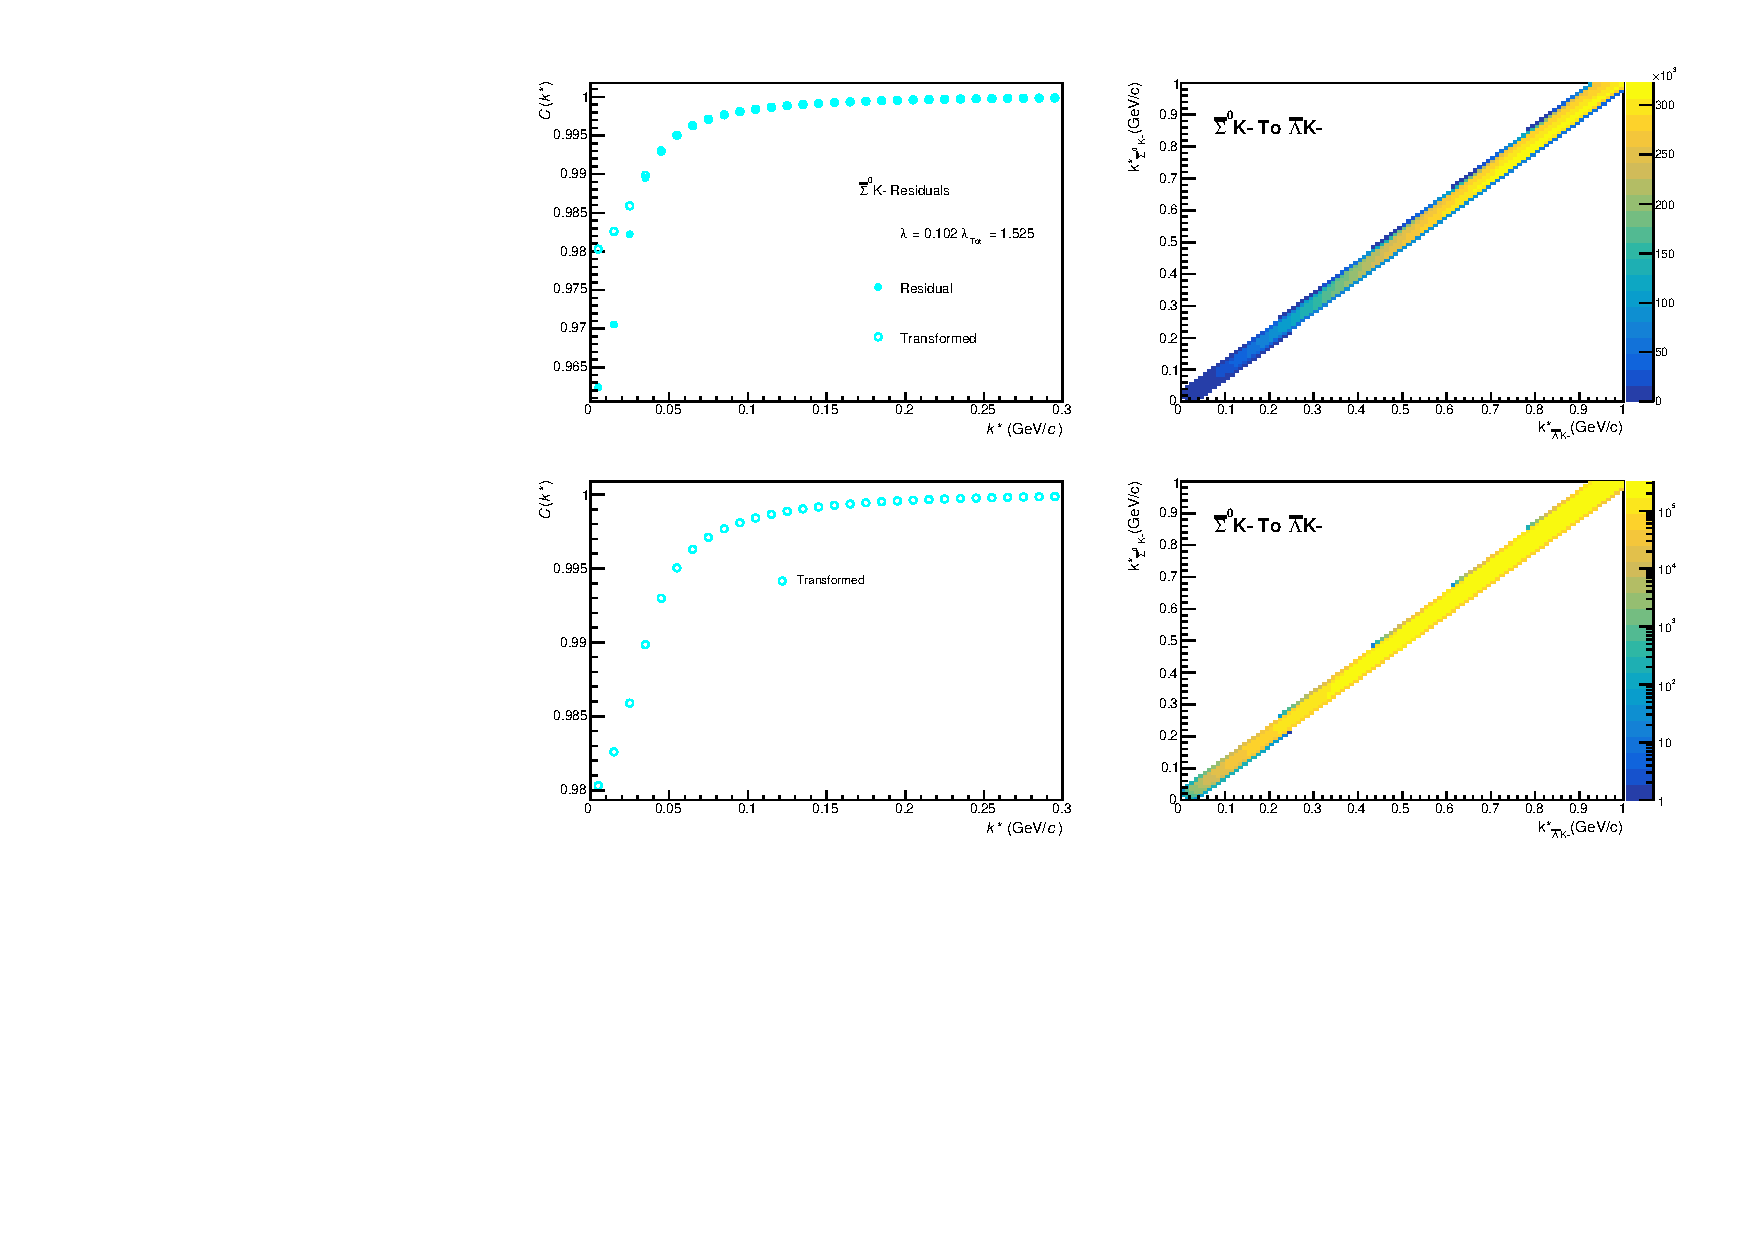
\includegraphics[width=\textwidth]{9_AdditionalFigures/Figures/Residuals/ALamKchM/Residuals_ALamKchM_0010_ASig0KchM_MomResCrctn_NonFlatBgdCrctn_10Res_PrimMaxDecay4fm_UsingXiDataAndCoulombOnly.pdf}
  \caption[Residuals: $\bar{\Sigma}^{0}$K$^{-}$ to $\bar{\Lambda}$K$^{-}$ (0-10\% Centrality)]{Residuals: $\bar{\Sigma}^{0}$K$^{-}$ to $\bar{\Lambda}$K$^{-}$ (0-10\% Centrality)}
  \label{fig:Res_ALamKchM_0010_ASig0KchM}
\end{figure}

\begin{figure}[h]
  \centering
  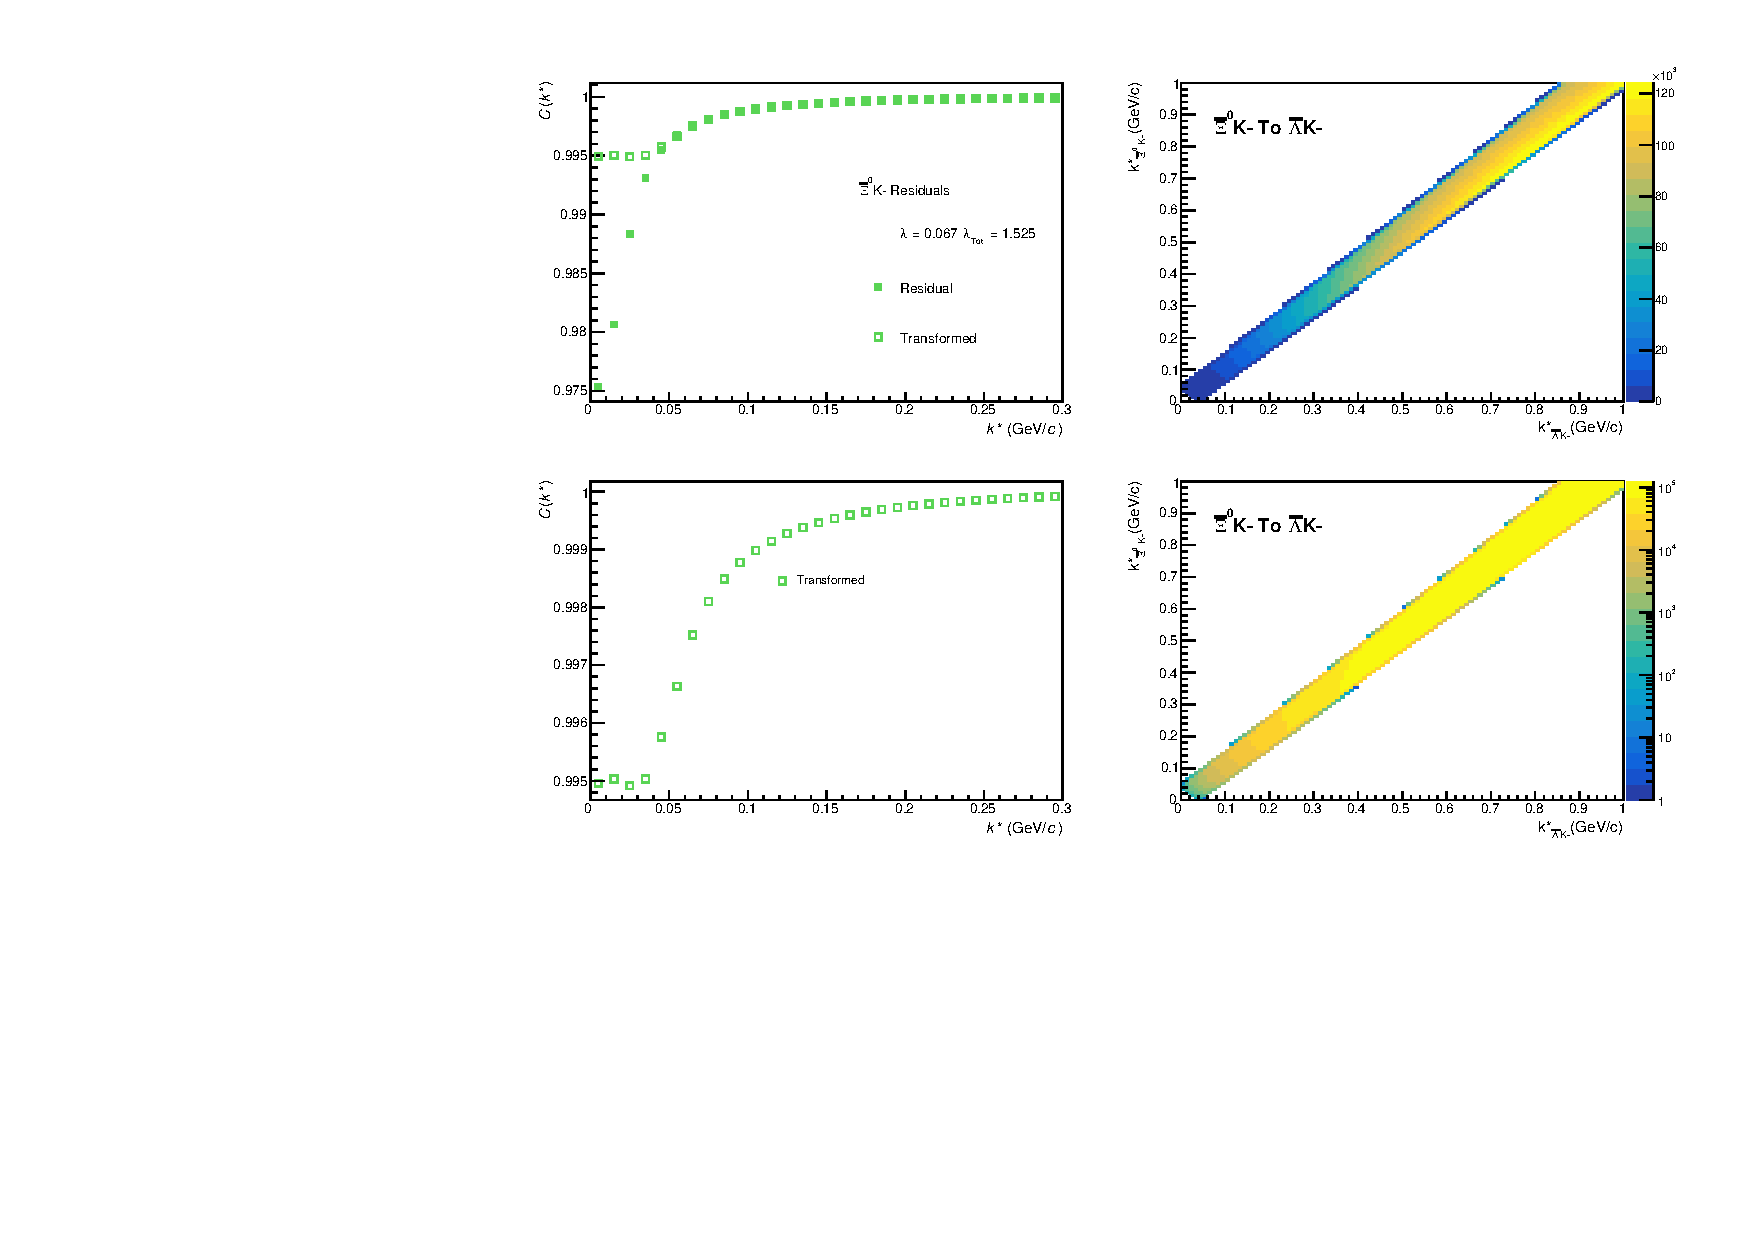
\includegraphics[width=\textwidth]{9_AdditionalFigures/Figures/Residuals/ALamKchM/Residuals_ALamKchM_0010_AXi0KchM_MomResCrctn_NonFlatBgdCrctn_10Res_PrimMaxDecay4fm_UsingXiDataAndCoulombOnly.pdf}
  \caption[Residuals: $\bar{\Xi}^{0}$K$^{-}$ to $\bar{\Lambda}$K$^{-}$ (0-10\% Centrality)]{Residuals: $\bar{\Xi}^{0}$K$^{-}$ to $\bar{\Lambda}$K$^{-}$ (0-10\% Centrality)}
  \label{fig:Res_ALamKchM_0010_AXi0KchM}
\end{figure}


\begin{figure}[h]
  \centering
  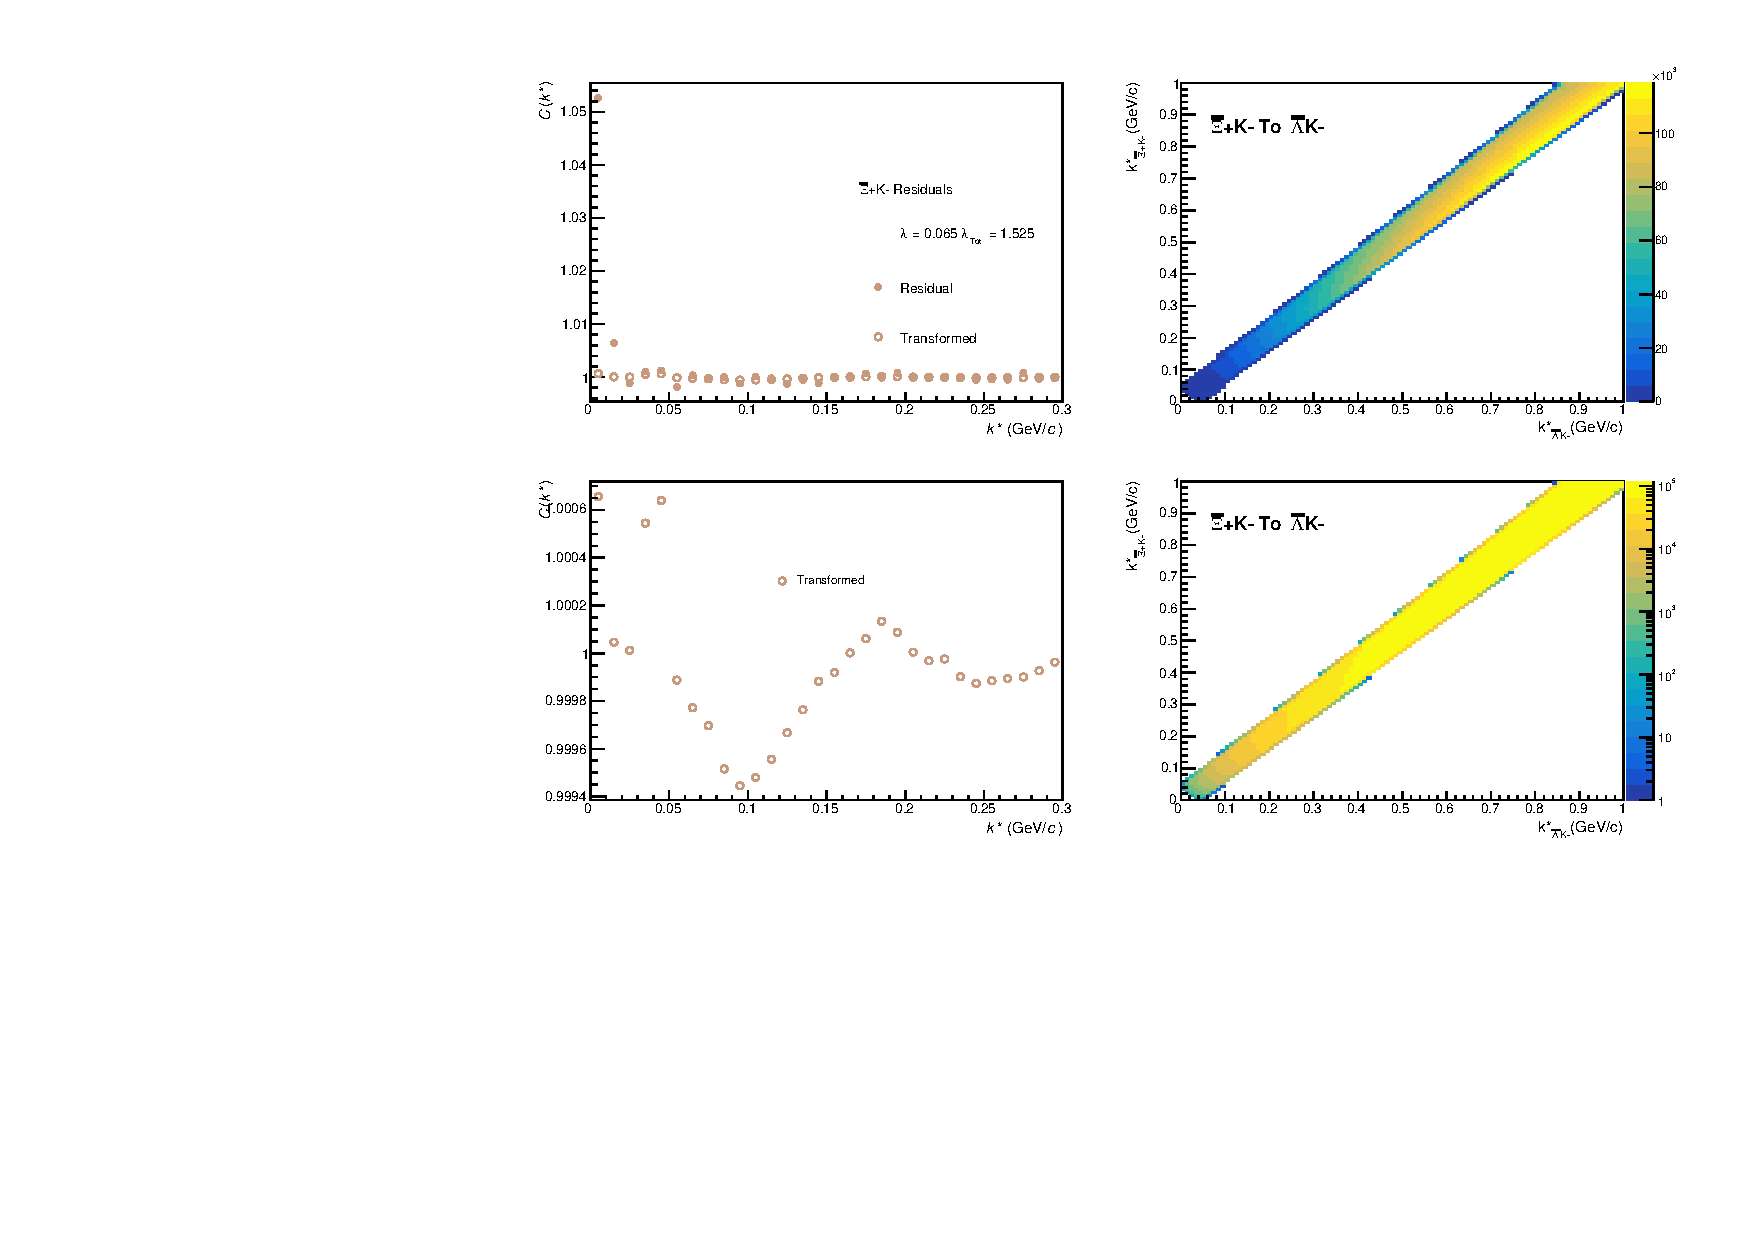
\includegraphics[width=\textwidth]{9_AdditionalFigures/Figures/Residuals/ALamKchM/Residuals_ALamKchM_0010_AXiKchM_MomResCrctn_NonFlatBgdCrctn_10Res_PrimMaxDecay4fm_UsingXiDataAndCoulombOnly.pdf}
  \caption[Residuals: $\bar{\Xi}^{+}$K$^{-}$ to $\bar{\Lambda}$K$^{-}$ (0-10\% Centrality)]{Residuals: $\bar{\Xi}^{+}$K$^{-}$ to $\bar{\Lambda}$K$^{-}$ (0-10\% Centrality)}
  \label{fig:Res_ALamKchM_0010_AXiCKchM}
\end{figure}


\begin{figure}[h]
  \centering
  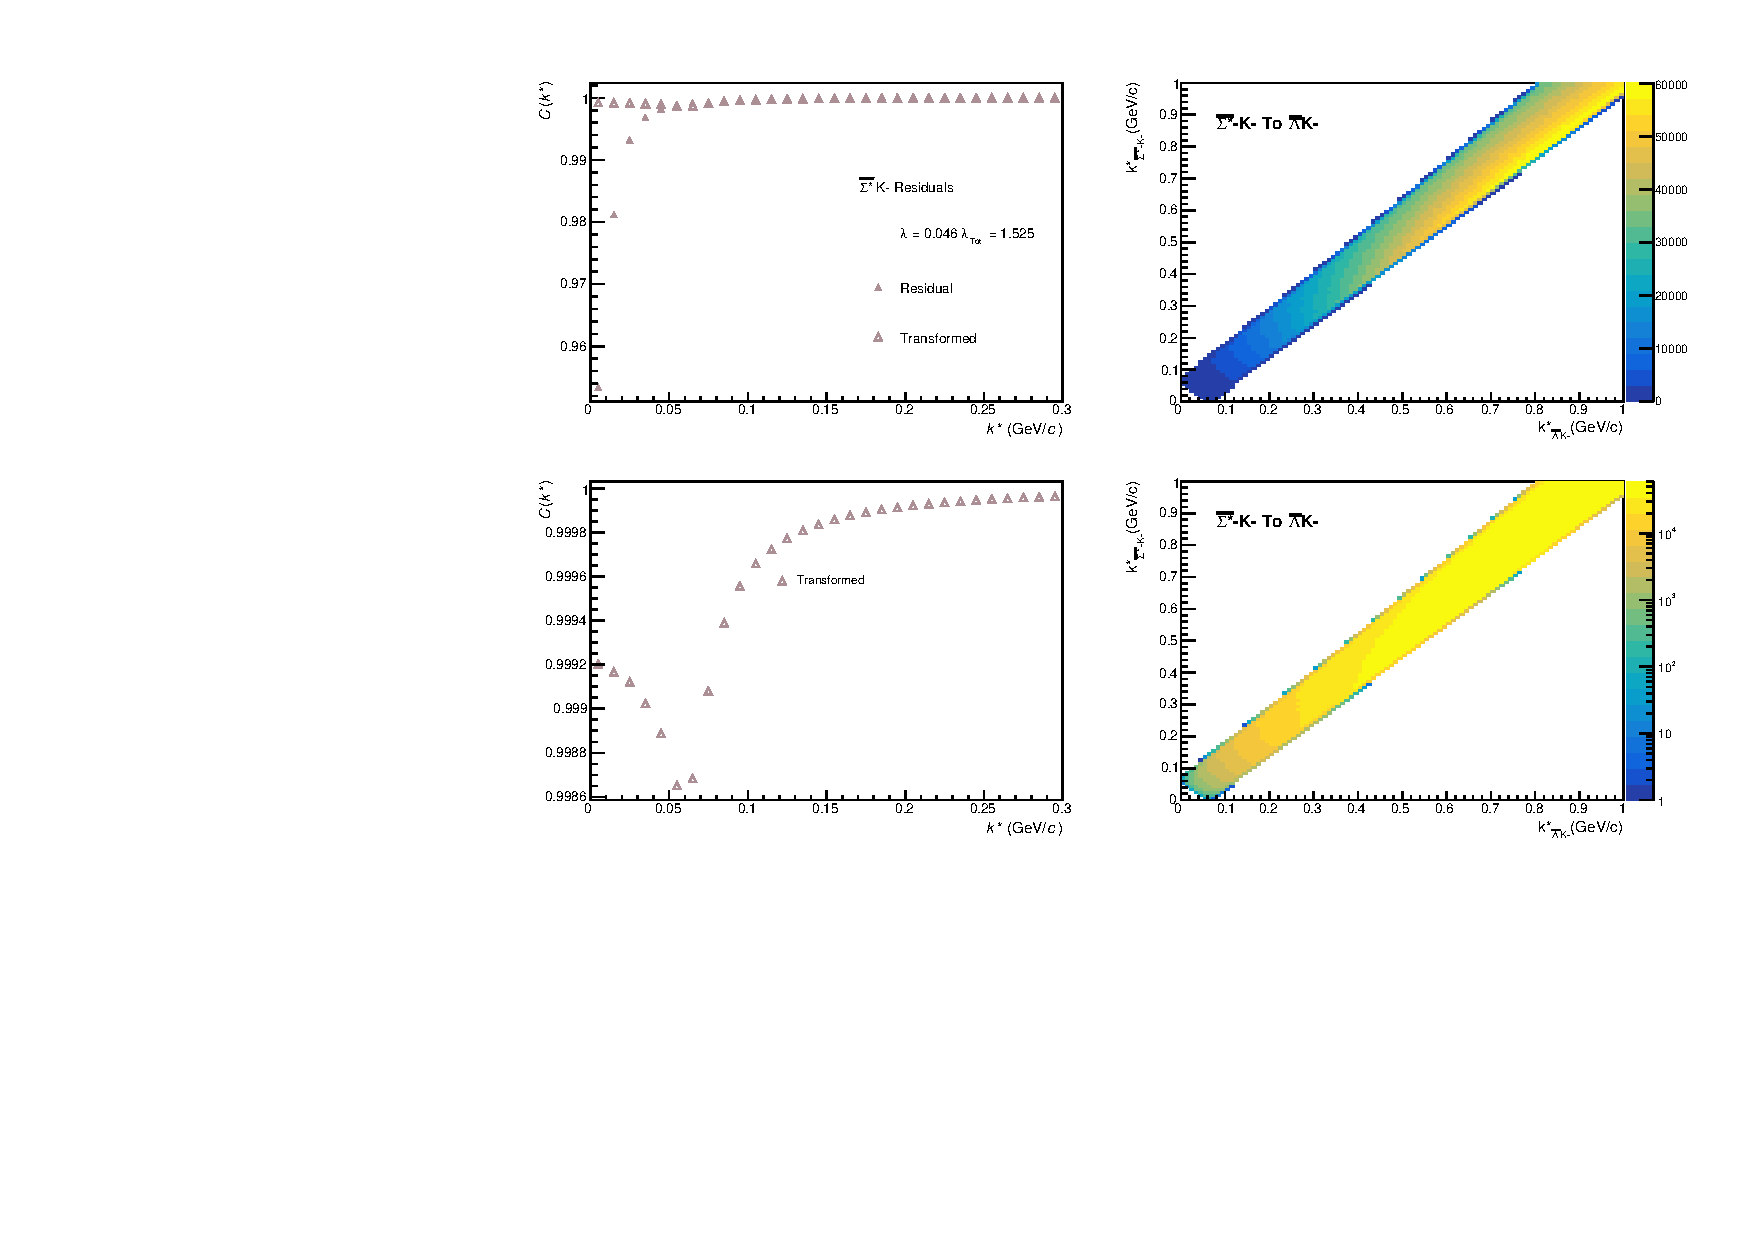
\includegraphics[width=\textwidth]{9_AdditionalFigures/Figures/Residuals/ALamKchM/Residuals_ALamKchM_0010_ASigStMKchM_MomResCrctn_NonFlatBgdCrctn_10Res_PrimMaxDecay4fm_UsingXiDataAndCoulombOnly.pdf}
  \caption[Residuals: $\bar{\Sigma}^{*-}$K$^{-}$ to $\bar{\Lambda}$K$^{-}$ (0-10\% Centrality)]{Residuals: $\bar{\Sigma}^{*-}$K$^{-}$ to $\bar{\Lambda}$K$^{-}$ (0-10\% Centrality)}
  \label{fig:Res_ALamKchM_0010_ASigStMKchM}
\end{figure}

\begin{figure}[h]
  \centering
  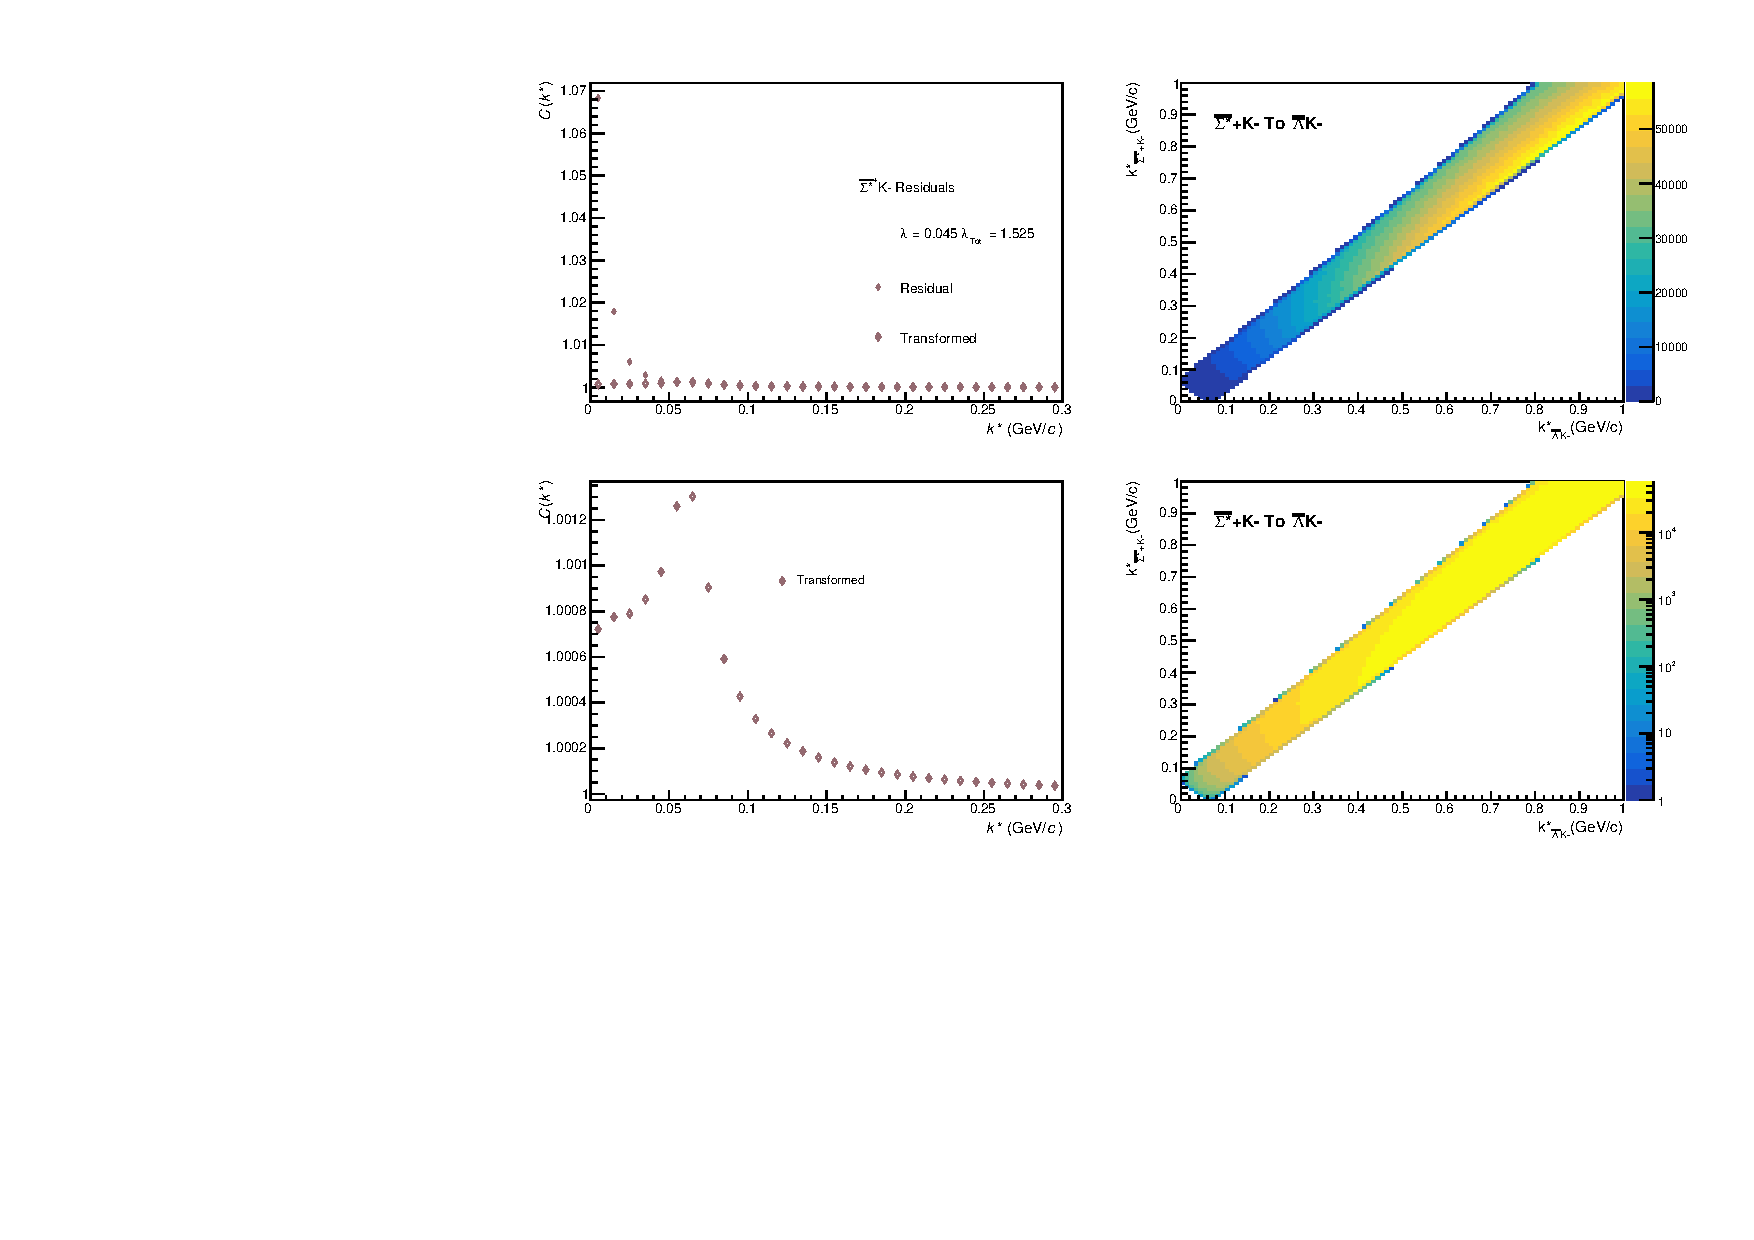
\includegraphics[width=\textwidth]{9_AdditionalFigures/Figures/Residuals/ALamKchM/Residuals_ALamKchM_0010_ASigStPKchM_MomResCrctn_NonFlatBgdCrctn_10Res_PrimMaxDecay4fm_UsingXiDataAndCoulombOnly.pdf}
  \caption[Residuals: $\bar{\Sigma}^{*+}$K$^{-}$ to $\bar{\Lambda}$K$^{-}$ (0-10\% Centrality)]{Residuals: $\bar{\Sigma}^{*+}$K$^{-}$ to $\bar{\Lambda}$K$^{-}$ (0-10\% Centrality)}
  \label{fig:Res_ALamKchM_0010_ASigStPKchM}
\end{figure}

\begin{figure}[h]
  \centering
  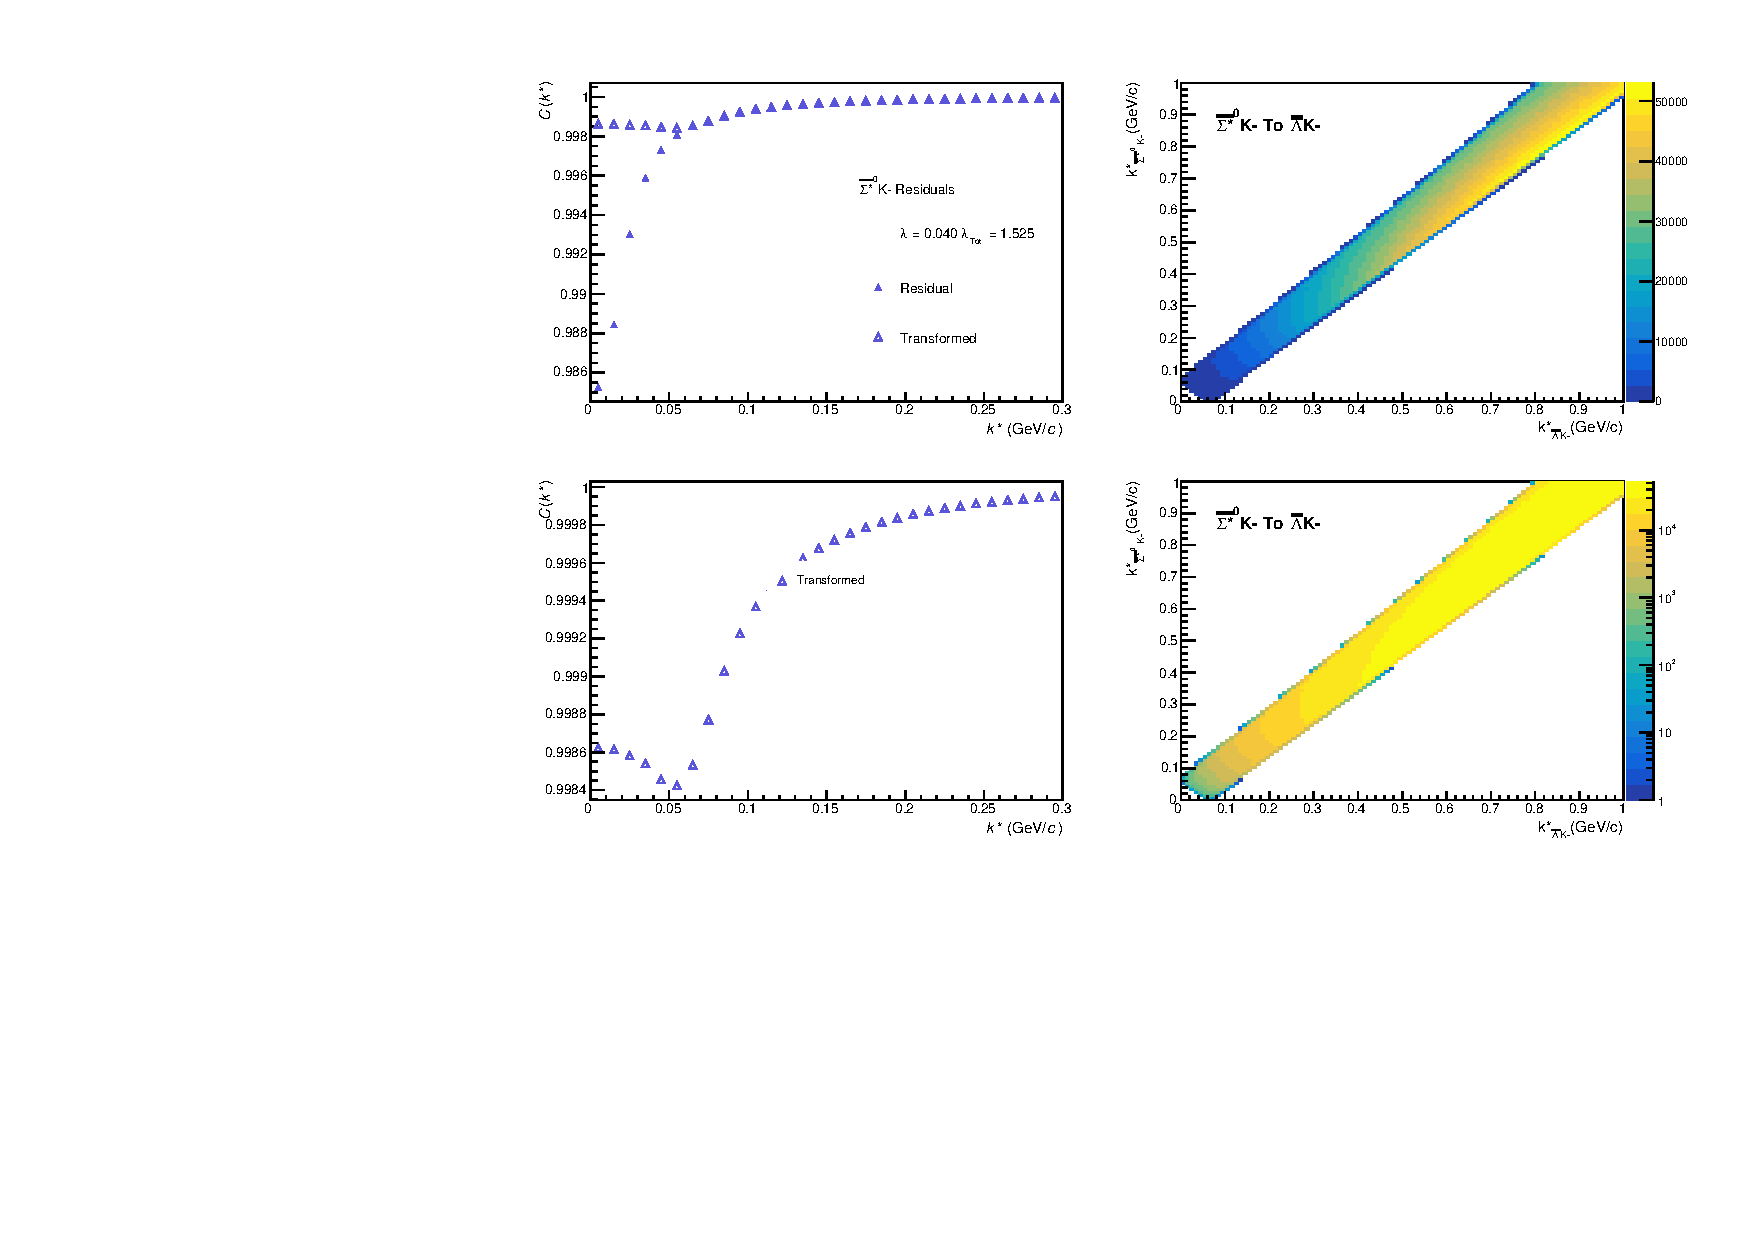
\includegraphics[width=\textwidth]{9_AdditionalFigures/Figures/Residuals/ALamKchM/Residuals_ALamKchM_0010_ASigSt0KchM_MomResCrctn_NonFlatBgdCrctn_10Res_PrimMaxDecay4fm_UsingXiDataAndCoulombOnly.pdf}
  \caption[Residuals: $\bar{\Sigma}^{*0}$K$^{-}$ to $\bar{\Lambda}$K$^{-}$ (0-10\% Centrality)]{Residuals: $\bar{\Sigma}^{*0}$K$^{-}$ to $\bar{\Lambda}$K$^{-}$ (0-10\% Centrality)}
  \label{fig:Res_ALamKchM_0010_ASigSt0KchM}
\end{figure}


\begin{figure}[h]
  \centering
  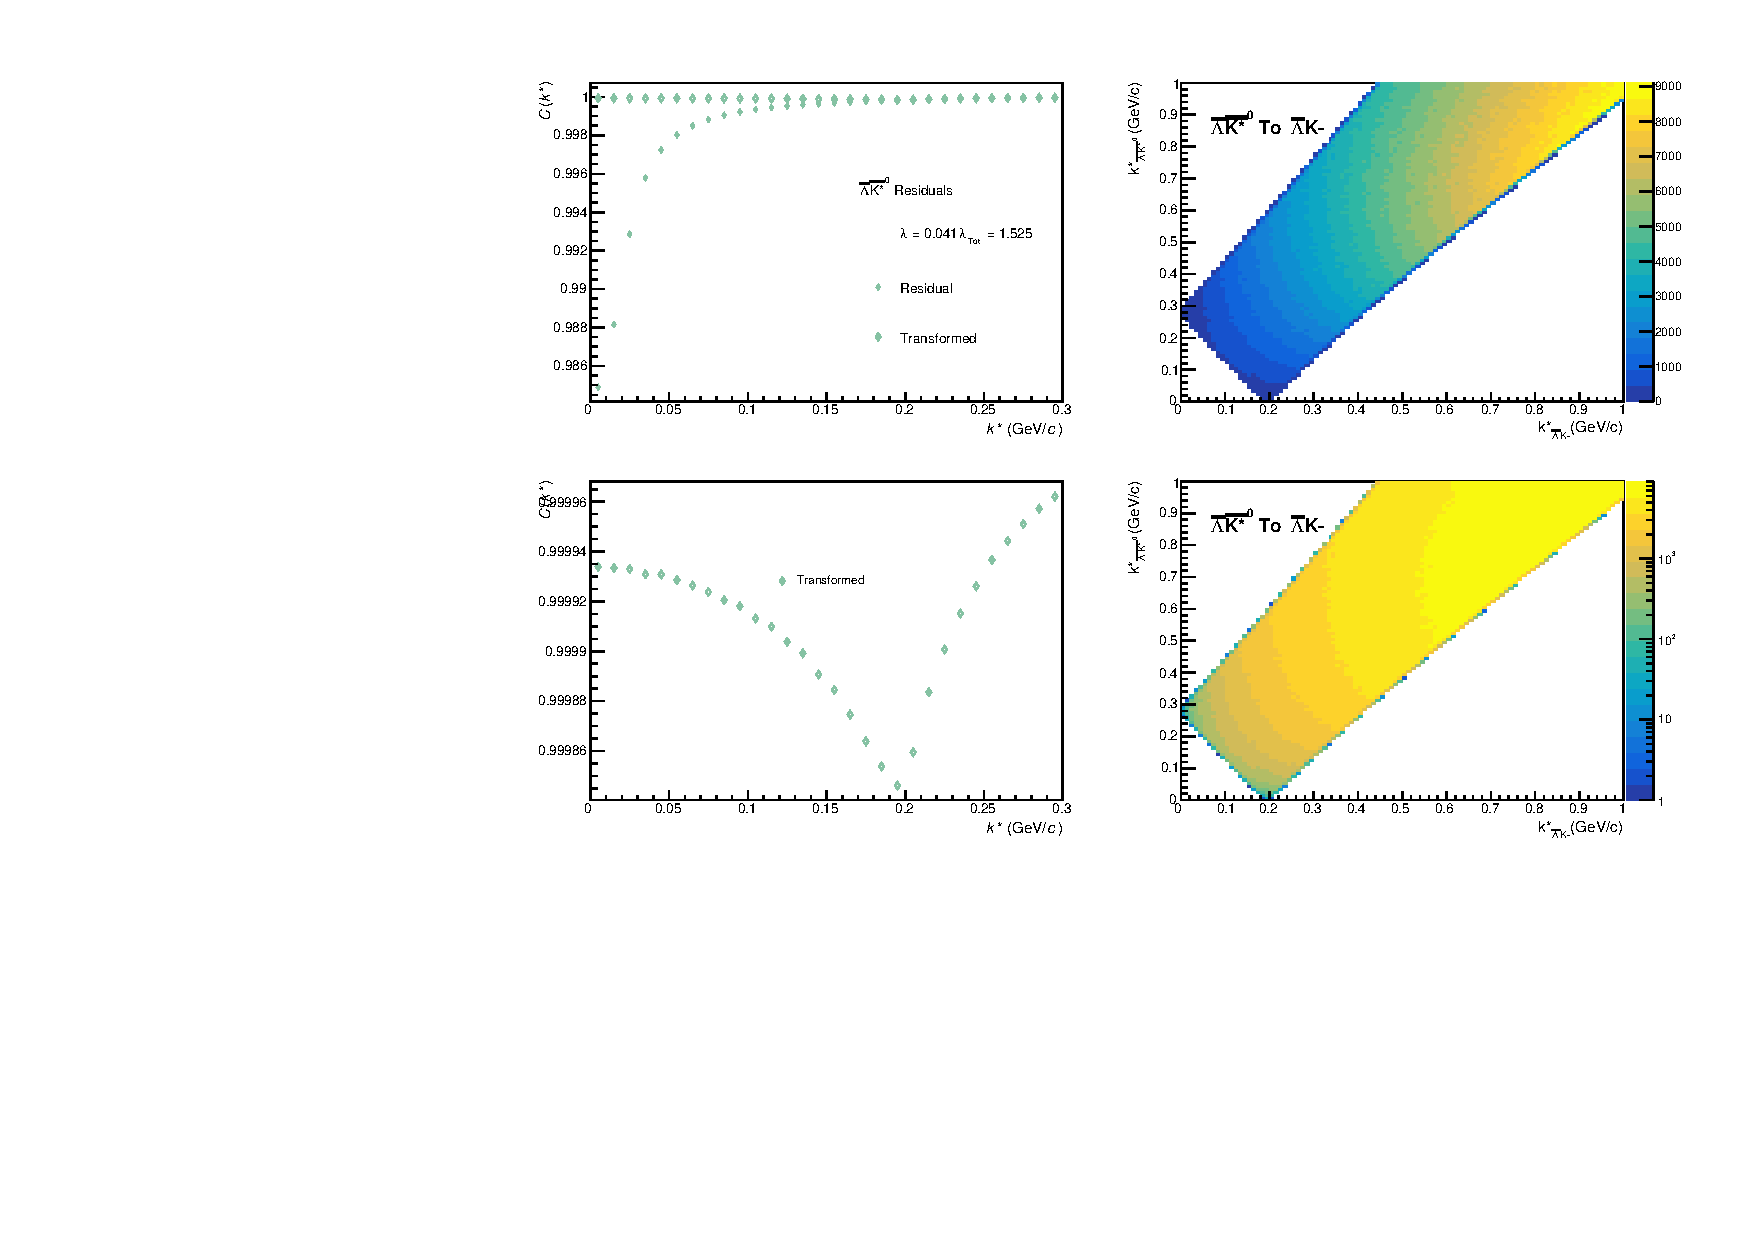
\includegraphics[width=\textwidth]{9_AdditionalFigures/Figures/Residuals/ALamKchM/Residuals_ALamKchM_0010_ALamAKSt0_MomResCrctn_NonFlatBgdCrctn_10Res_PrimMaxDecay4fm_UsingXiDataAndCoulombOnly.pdf}
  \caption[Residuals: $\bar{\Lambda}\bar{\mathrm{K}}^{*0}$ to $\bar{\Lambda}$K$^{-}$ (0-10\% Centrality)]{Residuals: $\bar{\Lambda}\bar{\mathrm{K}}^{*0}$ to $\bar{\Lambda}$K$^{-}$ (0-10\% Centrality)}
  \label{fig:Res_ALamKchM_0010_ALamAKSt0}
\end{figure}


\begin{figure}[h]
  \centering
  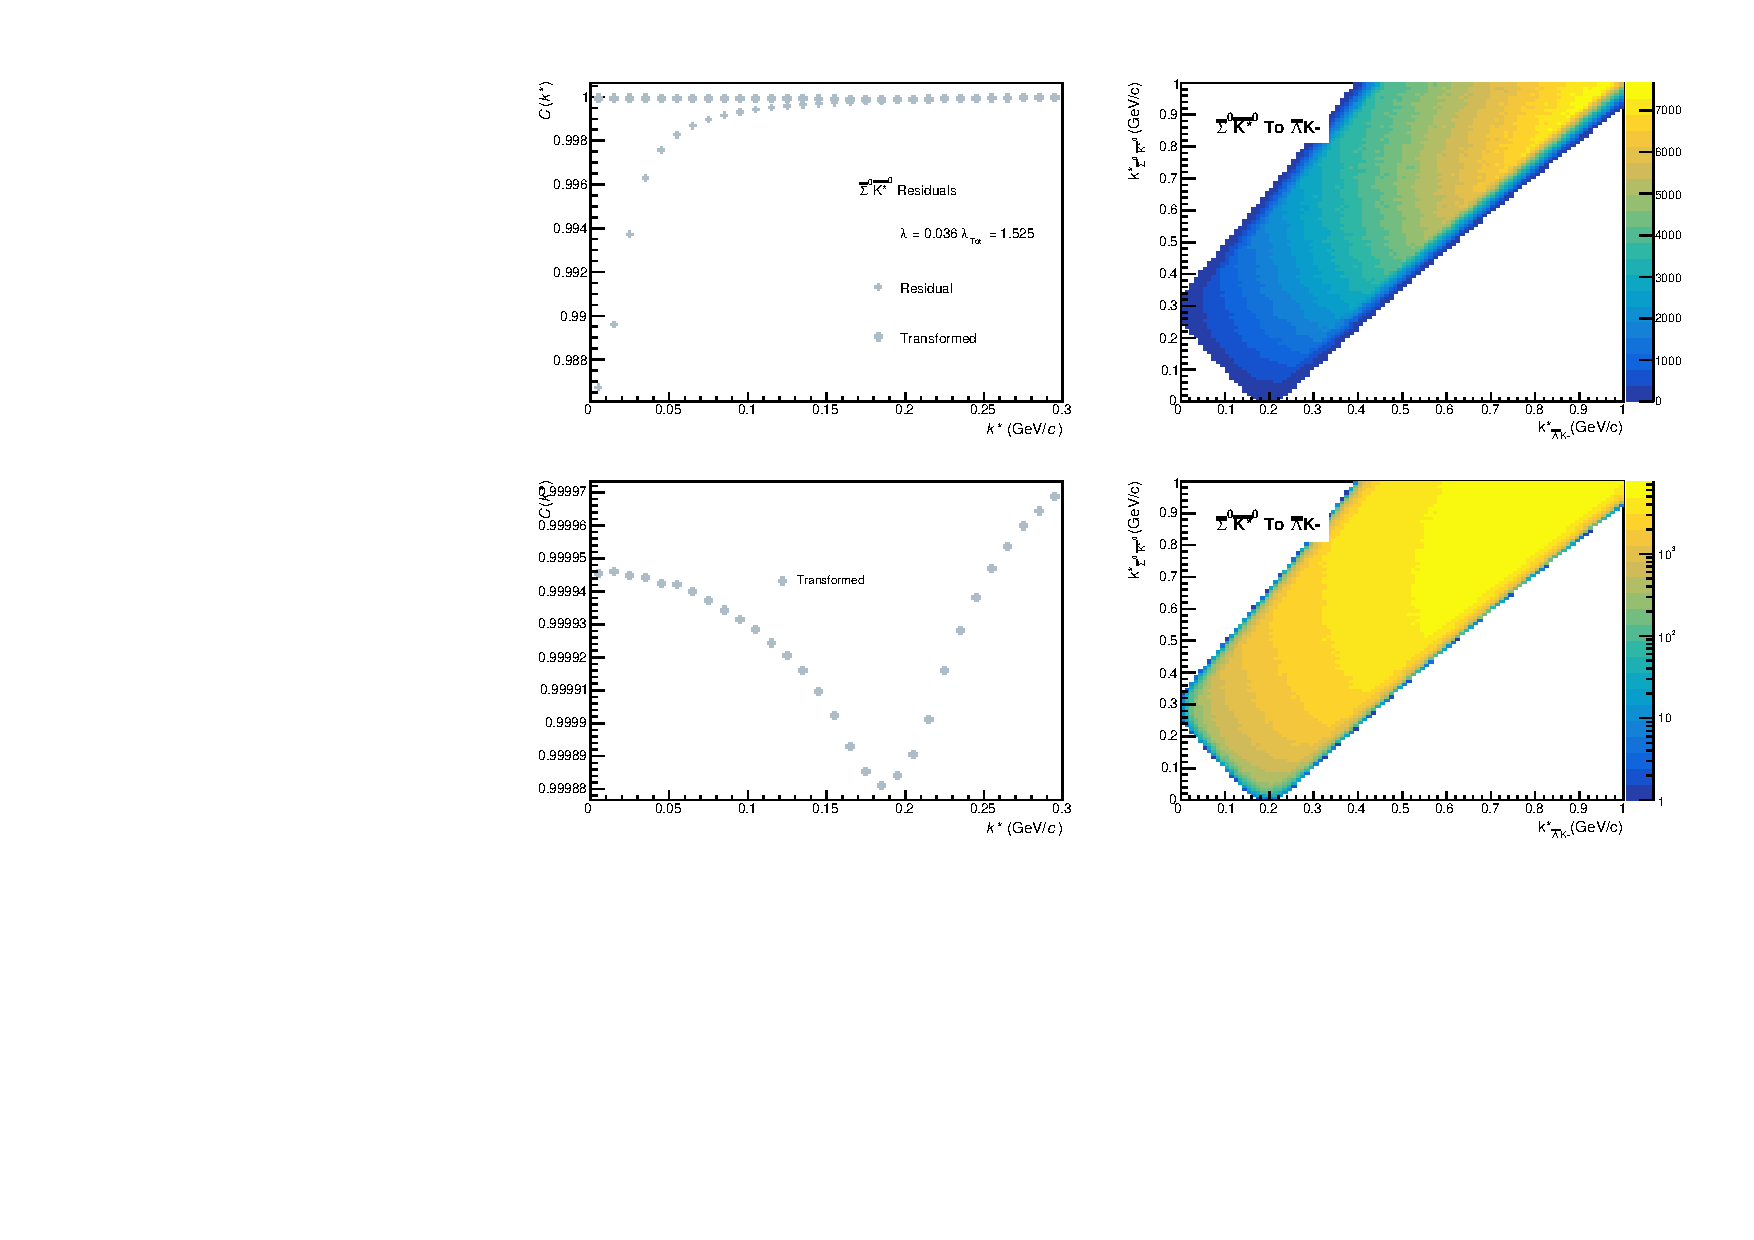
\includegraphics[width=\textwidth]{9_AdditionalFigures/Figures/Residuals/ALamKchM/Residuals_ALamKchM_0010_ASigma0AKSt0_MomResCrctn_NonFlatBgdCrctn_10Res_PrimMaxDecay4fm_UsingXiDataAndCoulombOnly.pdf}
  \caption[Residuals: $\bar{\Sigma}^{0}\bar{\mathrm{K}}^{*0}$ to $\bar{\Lambda}$K$^{-}$ (0-10\% Centrality)]{Residuals: $\bar{\Sigma}^{0}\bar{\mathrm{K}}^{*0}$ to $\bar{\Lambda}$K$^{-}$ (0-10\% Centrality)}
  \label{fig:Res_ALamKchM_0010_ASig0AKSt0}
\end{figure}


\begin{figure}[h]
  \centering
  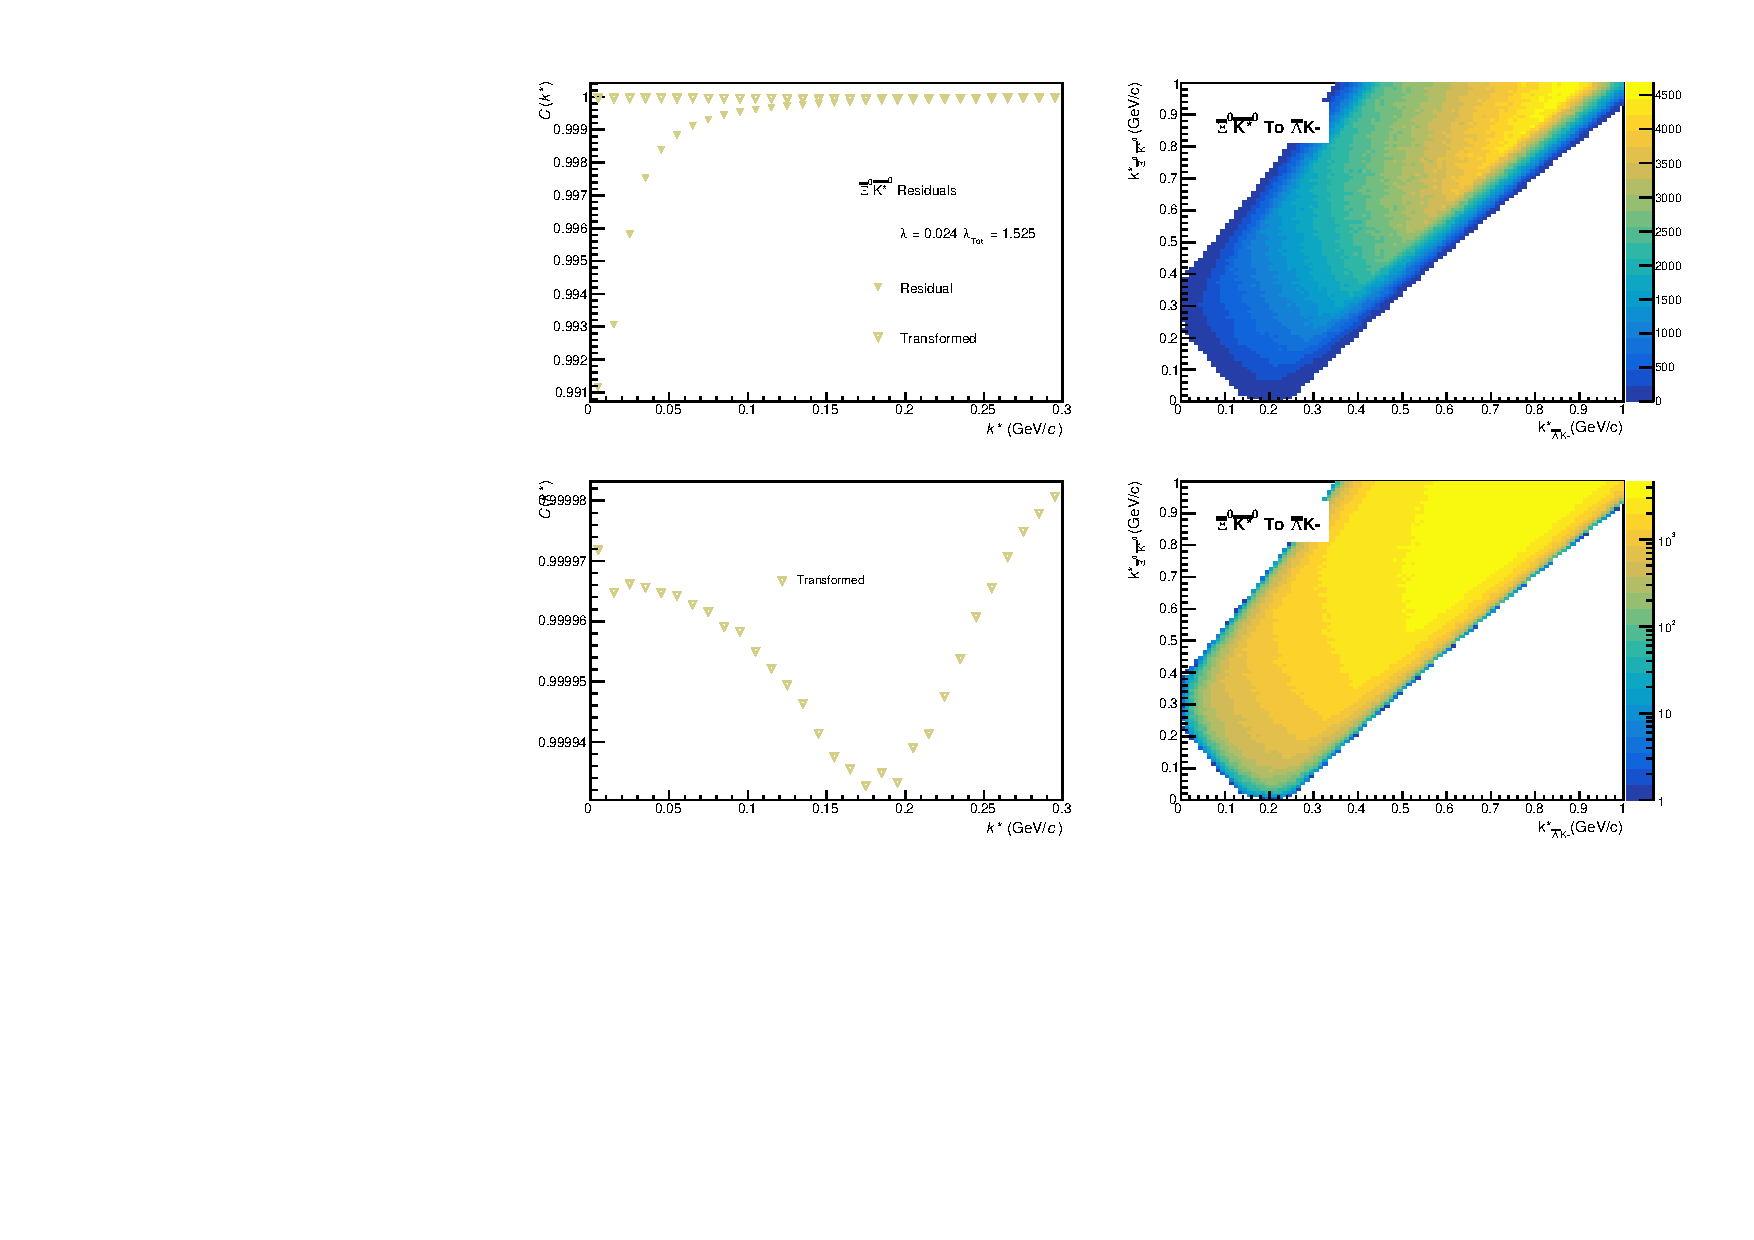
\includegraphics[width=\textwidth]{9_AdditionalFigures/Figures/Residuals/ALamKchM/Residuals_ALamKchM_0010_AXi0AKSt0_MomResCrctn_NonFlatBgdCrctn_10Res_PrimMaxDecay4fm_UsingXiDataAndCoulombOnly.pdf}
  \caption[Residuals: $\bar{\Xi}^{0}\bar{\mathrm{K}}^{*0}$ to $\bar{\Lambda}$K$^{-}$ (0-10\% Centrality)]{Residuals: $\bar{\Xi}^{0}\bar{\mathrm{K}}^{*0}$ to $\bar{\Lambda}$K$^{-}$ (0-10\% Centrality)}
  \label{fig:Res_ALamKchM_0010_AXi0AKSt0}
\end{figure}

\begin{figure}[h]
  \centering
  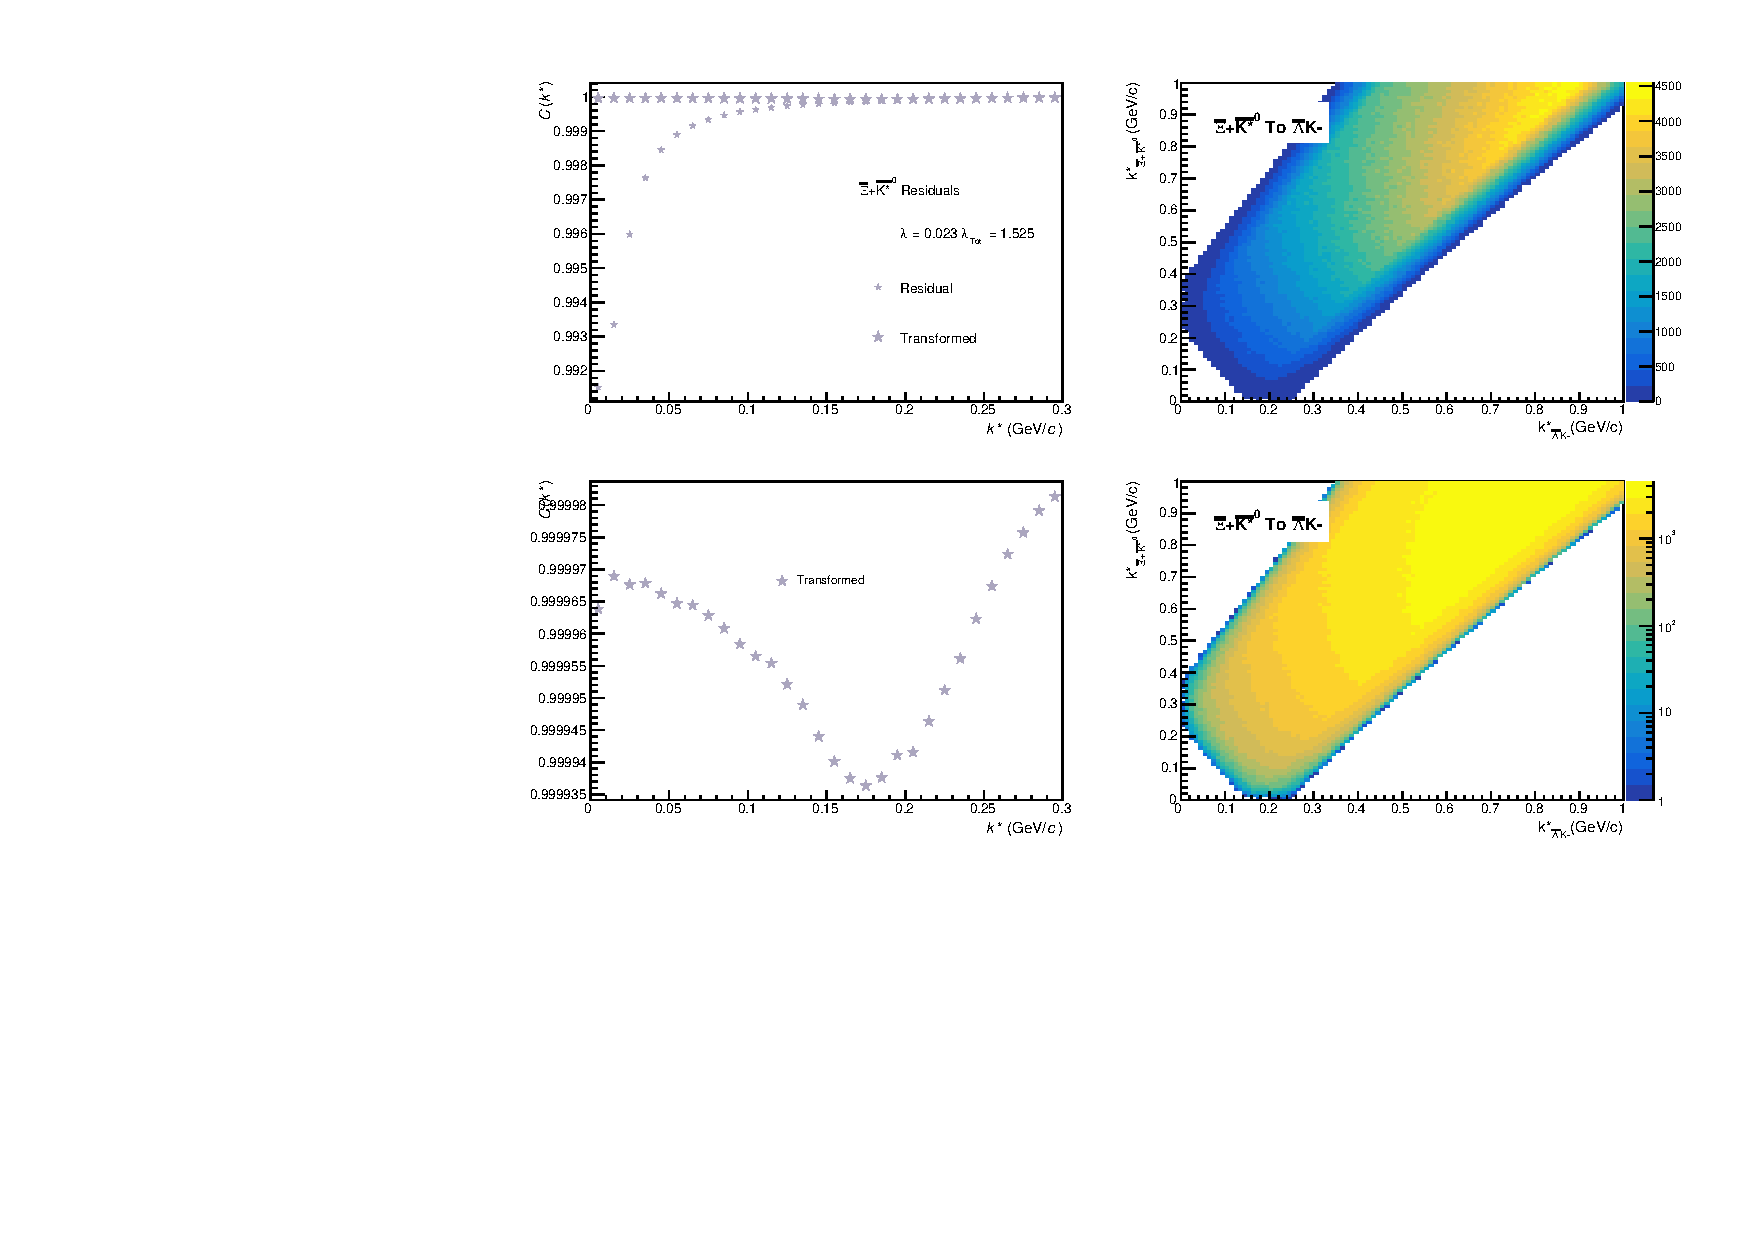
\includegraphics[width=\textwidth]{9_AdditionalFigures/Figures/Residuals/ALamKchM/Residuals_ALamKchM_0010_AXiAKSt0_MomResCrctn_NonFlatBgdCrctn_10Res_PrimMaxDecay4fm_UsingXiDataAndCoulombOnly.pdf}
  \caption[Residuals: $\bar{\Xi}^{+}\bar{\mathrm{K}}^{*0}$ to $\bar{\Lambda}$K$^{-}$ (0-10\% Centrality)]{Residuals: $\bar{\Xi}^{+}\bar{\mathrm{K}}^{*0}$ to $\bar{\Lambda}$K$^{-}$ (0-10\% Centrality)}
  \label{fig:Res_ALamKchM_0010_AXiCAKSt0}
\end{figure}


\end{document}